\documentclass{beamer}
\mode<presentation>
\usepackage{amsmath}
\usepackage{amssymb}
%\usepackage{advdate}
\usepackage{adjustbox}
\usepackage{subcaption}
\usepackage{enumitem}
\usepackage{multicol}
\usepackage{gensymb}
\usepackage{mathtools}
\usepackage{listings}
\usepackage{url}
\usepackage{hyperref}
\def\UrlBreaks{\do\/\do-}
\usetheme{Boadilla}
\usecolortheme{lily}
\setbeamertemplate{footline}
{
  \leavevmode%
  \hbox{%
  \begin{beamercolorbox}[wd=\paperwidth,ht=0.5ex,dp=0.5ex,right]{author in head/foot}%
    \insertframenumber{} / \inserttotalframenumber\hspace*{2ex} 
  \end{beamercolorbox}}%
  \vskip0pt%
}
\setbeamertemplate{navigation symbols}{}

\providecommand{\nCr}[2]{\,^{#1}C_{#2}} % nCr
\providecommand{\nPr}[2]{\,^{#1}P_{#2}} % nPr
\providecommand{\mbf}{\mathbf}
\providecommand{\pr}[1]{\ensuremath{\Pr\left(#1\right)}}
\providecommand{\qfunc}[1]{\ensuremath{Q\left(#1\right)}}
\providecommand{\sbrak}[1]{\ensuremath{{}\left[#1\right]}}
\providecommand{\lsbrak}[1]{\ensuremath{{}\left[#1\right.}}
\providecommand{\rsbrak}[1]{\ensuremath{{}\left.#1\right]}}
\providecommand{\brak}[1]{\ensuremath{\left(#1\right)}}
\providecommand{\lbrak}[1]{\ensuremath{\left(#1\right.}}
\providecommand{\rbrak}[1]{\ensuremath{\left.#1\right)}}
\providecommand{\cbrak}[1]{\ensuremath{\left\{#1\right\}}}
\providecommand{\lcbrak}[1]{\ensuremath{\left\{#1\right.}}
\providecommand{\rcbrak}[1]{\ensuremath{\left.#1\right\}}}
\theoremstyle{remark}
\newtheorem{rem}{Remark}
\newcommand{\sgn}{\mathop{\mathrm{sgn}}}
\providecommand{\abs}[1]{\left\vert#1\right\vert}
\providecommand{\res}[1]{\Res\displaylimits_{#1}} 
\providecommand{\norm}[1]{\lVert#1\rVert}
\providecommand{\mtx}[1]{\mathbf{#1}}
\providecommand{\mean}[1]{E\left[ #1 \right]}
\providecommand{\fourier}{\overset{\mathcal{F}}{ \rightleftharpoons}}
%\providecommand{\hilbert}{\overset{\mathcal{H}}{ \rightleftharpoons}}
\providecommand{\system}{\overset{\mathcal{H}}{ \longleftrightarrow}}
	%\newcommand{\solution}[2]{\textbf{Solution:}{#1}}
%\newcommand{\solution}{\noindent \textbf{Solution: }}
\providecommand{\dec}[2]{\ensuremath{\overset{#1}{\underset{#2}{\gtrless}}}}
\newcommand{\myvec}[1]{\ensuremath{\begin{pmatrix}#1\end{pmatrix}}}



\title{10.4.2.3}
\author{EE24BTECH11021 - Eshan Ray}
\date{\today}

\begin{document}

\begin{frame}
    \titlepage
\end{frame}

\begin{frame}
    \frametitle{Problem Statement}
    \textbf{Question:}\\
    Find two numbers whose sum is 27 and product is 182.
\end{frame}

\begin{frame}
    \frametitle{Solution 1: Using Algebra}
  Let one of the numbers be $x$\\
So, the other number is $27-x$\\
Given,
\begin{align}
    x\brak{27-x} &= 182\\
    27x-x^2 &=182\\
    x^2 - 27x + 182 &=0\\
    \brak{x-13}\brak{x-14} &= 0\\
    \implies    x &= 13,14
\end{align}
    So, the solutions are \( x = 13 \) and \( x = 14 \).
\end{frame}

\begin{frame}
    \frametitle{Computational Solution: Newton-Raphson Method}
    To find the roots of the quadratic equation \( x^2 - 27x + 182 = 0 \), we use the Newton-Raphson method.

\begin{align}
    x_{n+1} &= x_n - \frac{f\brak{x_n}}{f\prime\brak{x_n}}\\
    f\brak{x} &= x^2 - 27x +182\\
    f\prime\brak{x} &= 2x - 27\\
    x_{n+1} &= x_n - \frac{x_{n}^2-27x_n+182}{2x_n-27}
\end{align}
\end{frame}

\begin{frame}
    \frametitle{Computational Solution: Results}
    After running the Newton-Raphson method, we get the following roots:
    \begin{align}
        \text{Root 1:} & \ 14.00000000 \\
        \text{Root 2:} & \ 13.00000000
    \end{align}
\end{frame}
\begin{frame}
\frametitle{Newton Raphson Plot}
    \begin{center}
     %\centering
   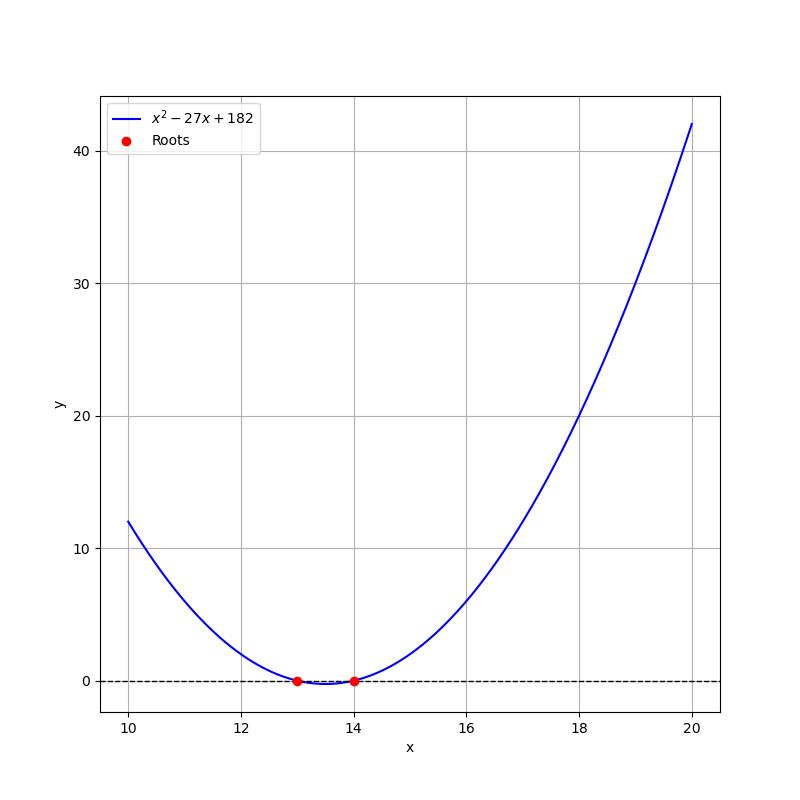
\includegraphics[width=0.7\textwidth]{plots/plot1.png}
        %\caption{Plot of the quadratic equation using Newton-Raphson method}
    \end{center}
\end{frame}

\begin{frame}
    \frametitle{Alternate Method: Eigenvalues of Companion Matrix}
   In this method, we find the roots of any polynomial of the form $x^n + a_{n-1}x^{n-1}\dots ax+a_0=0$ by finding the eigenvalues of the Companion Matrix $\brak{C}$ given below:-\\
\begin{align}
    C &= \myvec{0&1&0&\dots&0\\ 0&0&1&\dots&0\\ \vdots &\vdots &\vdots &\ddots&\vdots\\0&0&0&\vdots&1\\-a_0&-a_1&-a_2&\dots&-a_{n-1}}
\end{align}
For the Quadratic Equation $x^2-27x+182-0$, we get the following companion Matrix
\begin{align}
    C&=\myvec{0&1\\-182&27}
\end{align}
The roots of the equation is the eigenvalues of the matrix $C$ which has been calculated using the QR Decomposition process.
\end{frame}

\begin{frame}
    \frametitle{QR Decomposition : Gram-schmidt Process}
     In the QR Decomposition, the matrix $A$ is decomposed into matrices $Q$ and $R$ as:
    \begin{align}
    A&=QR
    \end{align}
    where ,$Q$ is an orthogonal matrix and $R$ is an upper triangular matrix.\\
     We start by producing an orthogonal set of column vectors of $Q$ \( \{ q_1, q_2, \dots, q_n \} \) from a set of column vectors of $A$ \( \{ a_1, a_2, \dots, a_n \} \).
     For orthogonalization we subtract each vector $a_i$ with the projections of all previously obtained orthogonal vectors $q_1,q_2,\dots,q_{i-1}$ to make $q_i$ orthogonal to them. \\
 \end{frame}
 \begin{frame}
    The projection of $a_i$ onto a vector $q_j$ is calculated as:
    \begin{align}
    proj_{q_j}(a_i) &= \frac{\langle a_i,q_j\rangle}{\langle q_j,q_j\rangle}q_j
    \end{align}
    Then $q_i$ is computed as:
    \begin{align}
    q_i &= a_i- \sum_{j=1}^{i-1}proj_{q_j}(a_i)
    \end{align}
    Then all the $q_i$'s are normalized by :
    \begin{align}
    q_i &= \frac{q_i}{||q_i||}
    \end{align}
    The process is repeated for all the colums of $A$
    \begin{enumerate}
    \item[3)] As $Q$ is an orthonormal matrix
    \begin{align}
        Q^\top Q &=I
    \end{align}
    So, $R$ can be represented as follows
    \begin{align}
        R &= Q^\top A\\
        r_{ij} &= \langle a_j, q_i \rangle \text{ , for  }  i \leq j 
    \end{align}
\end{enumerate}
\end{frame}

\begin{frame}
    \frametitle{QR Algorithm}
   In the  QR algorithm, the matrix $A_n$ is decomposed into matrices $Q_n$ and $R_n$ as:
    \begin{align}
    A_{n}&=Q_nR_n
    \end{align}
Then, the new matrix $A_{n+1}$ is computed as:
\begin{align}
A_{n+1}&=R_nQ_n
\end{align}
This process is repeated until the off-diagonal elements of the matrix become negligibly small, at which point the diagonal elements approximate the eigenvalues of the original matrix.
\end{frame}

\begin{frame}
    \frametitle{Eigenvalue Approach: Results}
    After applying the QR algorithm to the companion matrix, the eigenvalues are computed to be:
    \[
    \text{Eigenvalues:} \ 14.0, 13.0
    \]
 \end{frame}
 \begin{frame}
 \frametitle{Eigenvalue Approach Plot}
     \begin{center}
     %\centering
   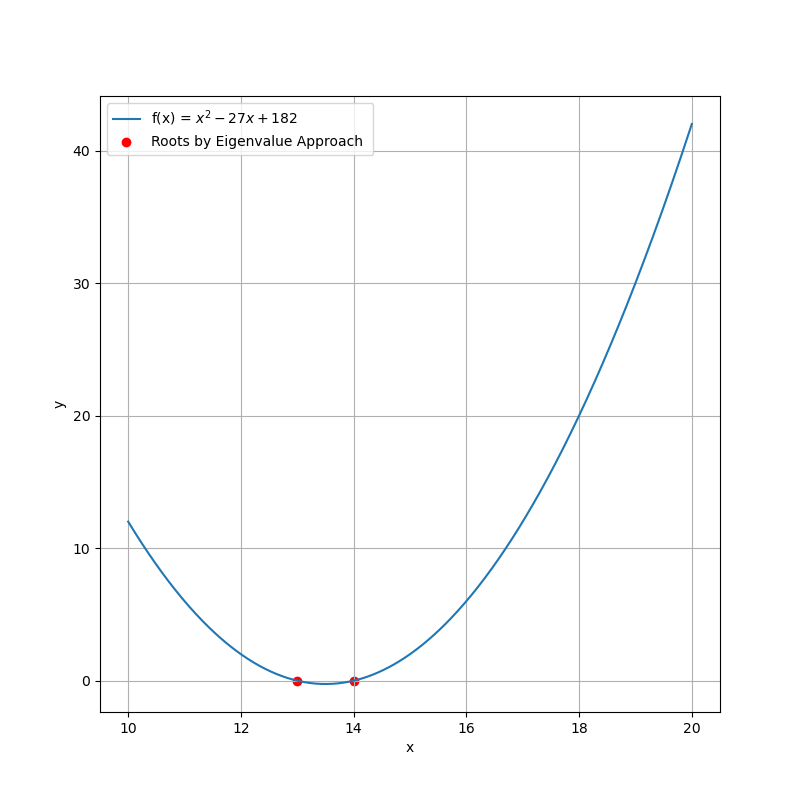
\includegraphics[width=0.7\textwidth]{plots/plot2.png}
        %\caption{Plot of the quadratic equation using Newton-Raphson method}
    \end{center}
\end{frame}

\begin{frame}
    \frametitle{Conclusion}
    \begin{itemize}
        \item The problem was solved using two methods: algebraic factorization and computational methods (Newton-Raphson and Eigenvalue approach).
        \item Both methods resulted in the same roots: \( 13 \) and \( 14 \).
        \item The eigenvalue method uses matrix operations to find roots, while Newton-Raphson provides a more direct approach.
    \end{itemize}
\end{frame}
\begin{frame}
    \frametitle{GitHub Repository}
   C code for Newton-Raphson:\\
    \url{https://github.com/eshan810/ee1003/blob/main/Assignments/5/codes/code.c} \\
    Python code for Newton-Raphson:\\
    \url{https://github.com/eshan810/ee1003/blob/main/Assignments/5/codes/root.py} \\
    C code for Eigenvalue Approach:\\
    \url{https://github.com/eshan810/ee1003/blob/main/Assignments/5/codes/eigen.c} \\
    Python code for Eigenvalue Approach:\\
    \url{https://github.com/eshan810/ee1003/blob/main/Assignments/5/codes/eigen.py}
    
\end{frame}

\end{document}

